\documentclass[12pt,]{article}
\usepackage[left=1in,top=1in,right=1in,bottom=1in]{geometry}
\newcommand*{\authorfont}{\fontfamily{phv}\selectfont}
\usepackage[]{libertine}


  \usepackage[T1]{fontenc}
  \usepackage[utf8]{inputenc}




\usepackage{abstract}
\renewcommand{\abstractname}{}    % clear the title
\renewcommand{\absnamepos}{empty} % originally center

\renewenvironment{abstract}
 {{%
    \setlength{\leftmargin}{0mm}
    \setlength{\rightmargin}{\leftmargin}%
  }%
  \relax}
 {\endlist}

\makeatletter
\def\@maketitle{%
  \newpage
%  \null
%  \vskip 2em%
%  \begin{center}%
  \let \footnote \thanks
    {\fontsize{18}{20}\selectfont\raggedright  \setlength{\parindent}{0pt} \@title \par}%
}
%\fi
\makeatother




\setcounter{secnumdepth}{0}

\usepackage{longtable,booktabs}



\title{EE282 Final Project Report \thanks{Replication files are
available on the author's Github account
(\url{http://github.com/ValentinaP-NYC}). \textbf{Current version}:
December 13, 2024; \textbf{Corresponding
author}:\href{mailto:valenp1@uci.edu}{\nolinkurl{valenp1@uci.edu}}.}  }
 



\author{\Large Valentina
Peña\vspace{0.05in} \newline\normalsize\emph{Nutritional Physiology Lab,
UC Irvine}  }


\date{}

\usepackage{titlesec}

\titleformat*{\section}{\normalsize\bfseries}
\titleformat*{\subsection}{\normalsize\itshape}
\titleformat*{\subsubsection}{\normalsize\itshape}
\titleformat*{\paragraph}{\normalsize\itshape}
\titleformat*{\subparagraph}{\normalsize\itshape}


\usepackage{natbib}
\bibliographystyle{apsr}
\usepackage[strings]{underscore} % protect underscores in most circumstances



\newtheorem{hypothesis}{Hypothesis}
\usepackage{setspace}


% set default figure placement to htbp
\makeatletter
\def\fps@figure{htbp}
\makeatother

\usepackage{hyperref}
\usepackage{array}
\usepackage{caption}
\usepackage{graphicx}
\usepackage{siunitx}
\usepackage[table]{xcolor}
\usepackage{multirow}
\usepackage{hhline}
\usepackage{calc}
\usepackage{tabularx}
\usepackage{fontawesome}
\usepackage[para,online,flushleft]{threeparttable}

% move the hyperref stuff down here, after header-includes, to allow for - \usepackage{hyperref}

\makeatletter
\@ifpackageloaded{hyperref}{}{%
\ifxetex
  \PassOptionsToPackage{hyphens}{url}\usepackage[setpagesize=false, % page size defined by xetex
              unicode=false, % unicode breaks when used with xetex
              xetex]{hyperref}
\else
  \PassOptionsToPackage{hyphens}{url}\usepackage[draft,unicode=true]{hyperref}
\fi
}

\@ifpackageloaded{color}{
    \PassOptionsToPackage{usenames,dvipsnames}{color}
}{%
    \usepackage[usenames,dvipsnames]{color}
}
\makeatother
\hypersetup{breaklinks=true,
            bookmarks=true,
            pdfauthor={Valentina Peña (Nutritional Physiology Lab, UC
Irvine)},
             pdfkeywords = {Fish physiology, nutrition,
transcriptomics},  
            pdftitle={EE282 Final Project Report},
            colorlinks=true,
            citecolor=blue,
            urlcolor=blue,
            linkcolor=magenta,
            pdfborder={0 0 0}}
\urlstyle{same}  % don't use monospace font for urls

% Add an option for endnotes. -----


% add tightlist ----------
\providecommand{\tightlist}{%
\setlength{\itemsep}{0pt}\setlength{\parskip}{0pt}}

% add some other packages ----------

% \usepackage{multicol}
% This should regulate where figures float
% See: https://tex.stackexchange.com/questions/2275/keeping-tables-figures-close-to-where-they-are-mentioned
\usepackage[section]{placeins}


\begin{document}
	
% \pagenumbering{arabic}% resets `page` counter to 1 
%    

% \maketitle

{% \usefont{T1}{pnc}{m}{n}
\setlength{\parindent}{0pt}
\thispagestyle{plain}
{\fontsize{18}{20}\selectfont\raggedright 
\maketitle  % title \par  

}

{
   \vskip 13.5pt\relax \normalsize\fontsize{11}{12} 
\textbf{\authorfont Valentina Peña} \hskip 15pt \emph{\small Nutritional
Physiology Lab, UC Irvine}   

}

}






\vskip -8.5pt


 % removetitleabstract

\noindent  

\section{METHODS}\label{methods}

\subsection{Experimental design}\label{experimental-design}

Liver paired-end raw sequencing files for all biological replicates of
\emph{Xiphister mucosus} and \emph{Phytichthys chirus} were obtained
from the original study {[}1{]} using SRA-tools v3.0.0 and the prefetch
tool from the SRA database. The downloaded .sra files were converted to
.fastq format using fasterq-dump, organizing the paired-end reads.
Following extraction, the .fastq files were compressed to .fastq.gz
format. The Bash script used for downloading and processing these files
is located at \emph{/code/ncbi\_download\_sequences\_submit.sh}, and the
raw reads are stored in \emph{/data/raw/fastq}.

\subsection{Pre-assembly quality
control}\label{pre-assembly-quality-control}

Quality reports for the raw read data were generated for each sample
using FastQC {[}2{]} and aggregated into a single report with MultiQC
{[}3{]}. These reports are located at: \emph{data/raw/fastqc\_results}.
After inspecting the reports, adapter contamination and low-quality base
calls were removed using Fastp {[}4{]}, which produced individual
quality reports for each sample, post-trimming. The trimming Bash script
is located at \emph{data/raw/fastq/fastp\_job.sh}. The post-trimming
reports and high-quality cleaned reads are stored in
\emph{output/reports/fastp} and \emph{data/processed/trimmed\_out},
respectively.

\subsection{De novo transcriptome assembly and
annotation}\label{de-novo-transcriptome-assembly-and-annotation}

Following the approach of Herrera et al.~(2022), transcriptome
assemblies were conducted using Trinity v2.15.2 {[}5{]}. RNA-seq data
for X.mucosus and P.chirus were processed separately to produce
species-specific assemblies. Each assembly incorporated pooled RNA-seq
data across experimental conditions to maximize transcript diversity.
Trinity performed \emph{in silico normalization} of reads to reduce
systematic coverage and improve assembly performance. Batch jobs were
submitted using custom scripts located at \emph{code/scripts}. The
script TrinityStats.pl was utilized to summarize basic metrics for the
P.chirus and X.mucosus \emph{de novo} assemblies which can be found in
\emph{output/reports}.

Prefixes `pc' and `xm' were used throughout the final project directory
to distinguish sub-directories and files for P.chirus and X.mucosus,
respectively. For example, Trinity outputs for P. chirus and X.mucosus
are found in \emph{data/processed/pc\_trinity\_out.Trinity.fasta.gz}
\emph{data/processed/xm\_trinity\_out.Trinity.fasta.gz}.

Transcriptome annotation was performed using Trinotate v4.0.2 {[}6{]}.
Open reading frames (ORFs) were identified using TransDecoder v2.0.1
{[}7{]}, and translated ORFs were aligned against the Swiss-Prot
database using BLASTX. The best hits were annotated with Gene Ontology
(GO) terms. Protein domains were identified with HMMER v3.1 and hmmscan
against the Pfam-A database. Individual Trinotate reports were generated
for each species and are located at
\emph{output/reports/pc\_debugged\_trinotate.xls} and
\emph{output/reports/xm\_Trinotate.sqlite/xm\_debugged\_trinotate.xls}.

\subsection{Transcript differential expression and enrichment
analysis}\label{transcript-differential-expression-and-enrichment-analysis}

Reads were aligned to the de novo assembled contigs using Bowtie2
{[}8{]}, and transcript abundance was quantified with RSEM, enabling
isoform- and gene-level quantification by clustering transcripts
representing splicing isoforms {[}9{]}. Relative expression was reported
as fragments per kilobase of transcript per million mapped reads (FPKM).
Downstream analyses focused on the \emph{pc\_all} and \emph{xm\_all}
matrix outputs, located in \emph{data/processed/abundances}.

Differential expression analysis was conducted using the combined
replicates \emph{all.isoform.counts. matrix} file for each species to
identify differentially expressed transcript isoforms across dietary
conditions. Analysis was performed with EdgeR implemented with Trinity,
using an FDR cutoff of 0.01, and transcripts with a fold change greater
than 2.5 were classified as significantly differentially expressed
{[}10{]}. Gene Ontology (GO) enrichment analysis of the differentially
expressed transcript isoforms was performed using GOseq, accounting for
gene length bias {[}11{]}. Biological sample quality was assessed with
the Trinity PtR script, which generated PCA plots to evaluate clustering
of individuals within each species across dietary conditions. The
outputs are located in: \emph{data/processed/edgeR/pc},
\emph{data/processed/edgeR/xm}, and \emph{data/processed/edgeR/PtR}. The
code to conduct the analysis can be located at:
\emph{data/processed/edgeR/edgeR\_script.R}.

\section{RESULTS}\label{results}

\subsection{Principle component
analysis}\label{principle-component-analysis}

For P.chirus, PC1 explains 72.57\% of the total variance, followed by
PC2 with 18.50\% and PC3 with 8.93\% (Fig.2A-B). A heatmap of the top 50
features contributing to variance in PC2 demonstrate clearer clustering
of replicates within dietary conditions, based on isoform-level
expression (Supplemtary material S1). This indicates that isoform
expression in P. chirus was influenced by dietary conditions to a
notable extent. Additional support for this can be noted in the total
number of unique DE transcripts which is 1812

In X.mucosus, 37.61\% of the total variance is explained by the first
principal component (PC1), with PC2 accounting for 27.99\%, and PC3
capturing an additional 17.88\% (Fig.2C-D). Heatmaps of the top 50
features contributing to variance in PC1, PC2, and PC3, respectively,
reveal that replicates within dietary conditions do not cluster
distinctly. This observation suggests that isoform-level expression in
X.mucosus is not strongly influenced by dietary condition. Across all
three dietary conditions there were only 290 DE transcripts at the
criteria (FDR \textless{} 0.01) and FC \textgreater{} 2.5.

\begin{figure}[htbp]
\centering
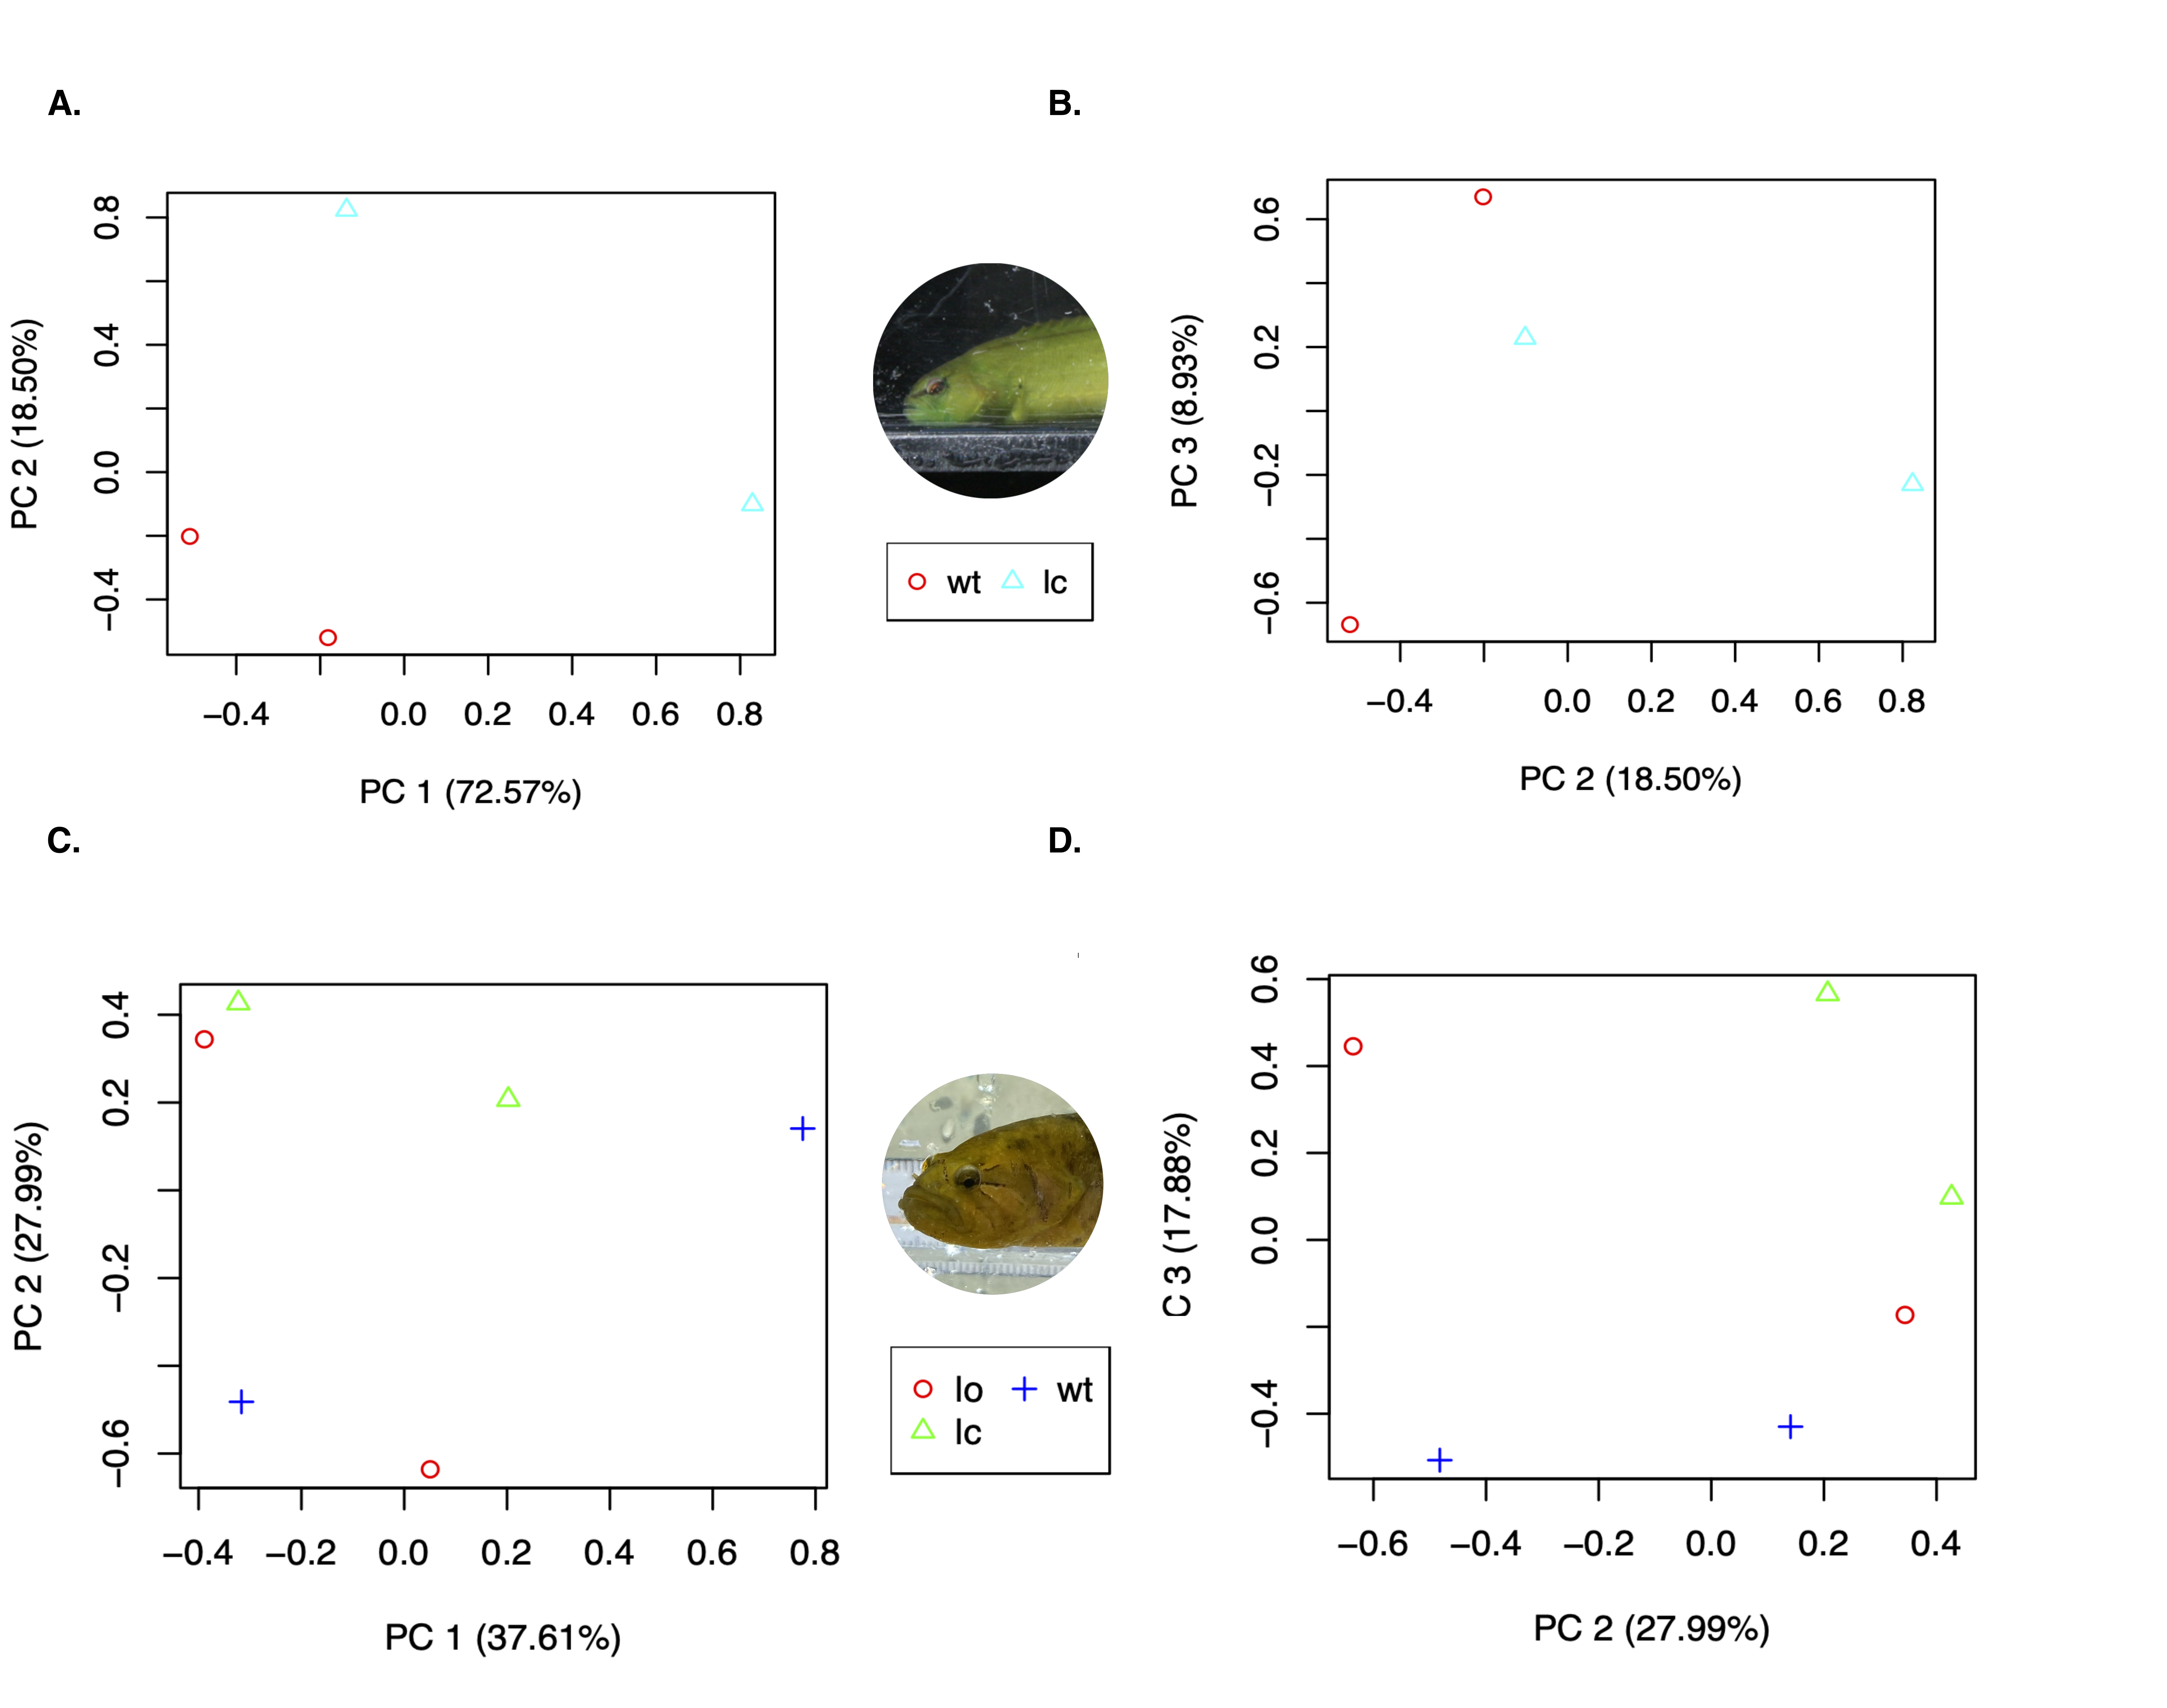
\includegraphics[width=0.85\textwidth]{output/figures/pc_and_xm_TMM_EXPR.minRow10.log2.centered.prcomp.principal_components.png}
\caption{Principle components (PCA) plot for (A-B) P.chirus (n=4) and (C-D) X.mucosus (n=6). Replicates within a species are colored according to dietary treatment (lo = lab-omnivore; lc = lab-carnivore; wt = wild-type/no dietary intervention.) Lowly expressed transcripts (< 0.5 CPM) were not considered.}
\end{figure}

\subsection{Transcriptome assembly and
annotation}\label{transcriptome-assembly-and-annotation}

Transcripts were subjected to annotation analysis by comparing with Nr,
Nt, Pfam, Swiss-Prot, KEGG and GO databases. Trinotate result summary
shows approximately 38\% of unique genes in P.chirus and 43\% of unique
genes in X.mucosus were assigned Pfam IDs during annotation. Annotation
revealed 6,172 Pfam domains in P. chirus and 5,369 in X. mucosus for
unique genes Table 1). For total genes, P.chirus had 65,691 Pfam IDs,
while X. mucosus had 55,925.

\begin{longtable}[]{@{}
  >{\raggedright\arraybackslash}p{(\columnwidth - 8\tabcolsep) * \real{0.1293}}
  >{\raggedright\arraybackslash}p{(\columnwidth - 8\tabcolsep) * \real{0.1973}}
  >{\raggedright\arraybackslash}p{(\columnwidth - 8\tabcolsep) * \real{0.2381}}
  >{\raggedright\arraybackslash}p{(\columnwidth - 8\tabcolsep) * \real{0.1973}}
  >{\raggedright\arraybackslash}p{(\columnwidth - 8\tabcolsep) * \real{0.2381}}@{}}
\toprule\noalign{}
\begin{minipage}[b]{\linewidth}\raggedright
Species
\end{minipage} & \begin{minipage}[b]{\linewidth}\raggedright
P.chirus (Unique)
\end{minipage} & \begin{minipage}[b]{\linewidth}\raggedright
P.chirus (Total)
\end{minipage} & \begin{minipage}[b]{\linewidth}\raggedright
X.mucosus (Unique)
\end{minipage} & \begin{minipage}[b]{\linewidth}\raggedright
X.mucosus (Total)
\end{minipage} \\
\midrule\noalign{}
\endhead
\bottomrule\noalign{}
\endlastfoot
Pfam & 6172 & 65691 & 5369 & 55925 \\
Genes & 16126 & 30076 & 13007 & 23304 \\
Transcripts & 26181 & 49723 & 23402 & 42952 \\
Proteins & 28588 & 51160 & 25891 & 44524 \\
\end{longtable}

Table 1: Pfam summarized Trinotate reporting. Annotated features (unique
and total) for X.mucosus and P.chirus assemblies.

\subsection{Transcript-level quantification and differential expression
analysis}\label{transcript-level-quantification-and-differential-expression-analysis}

In this study, liver RNA-seq data from X. mucosus and P. chirus were
analyzed to assess differential isoform-level expression in response to
dietary conditions. The objective was to explore how diet-induced
changes influence gene expression, focusing on alternative isoform
usage. Transcript abundance was quantified using RSEM, and differential
expression (DE) analysis was conducted in EdgeR with an FDR
\textless0.01 and a fold change (FC) \textgreater2.5 across all pairwise
comparisons.

\begin{figure}[htbp]
\centering
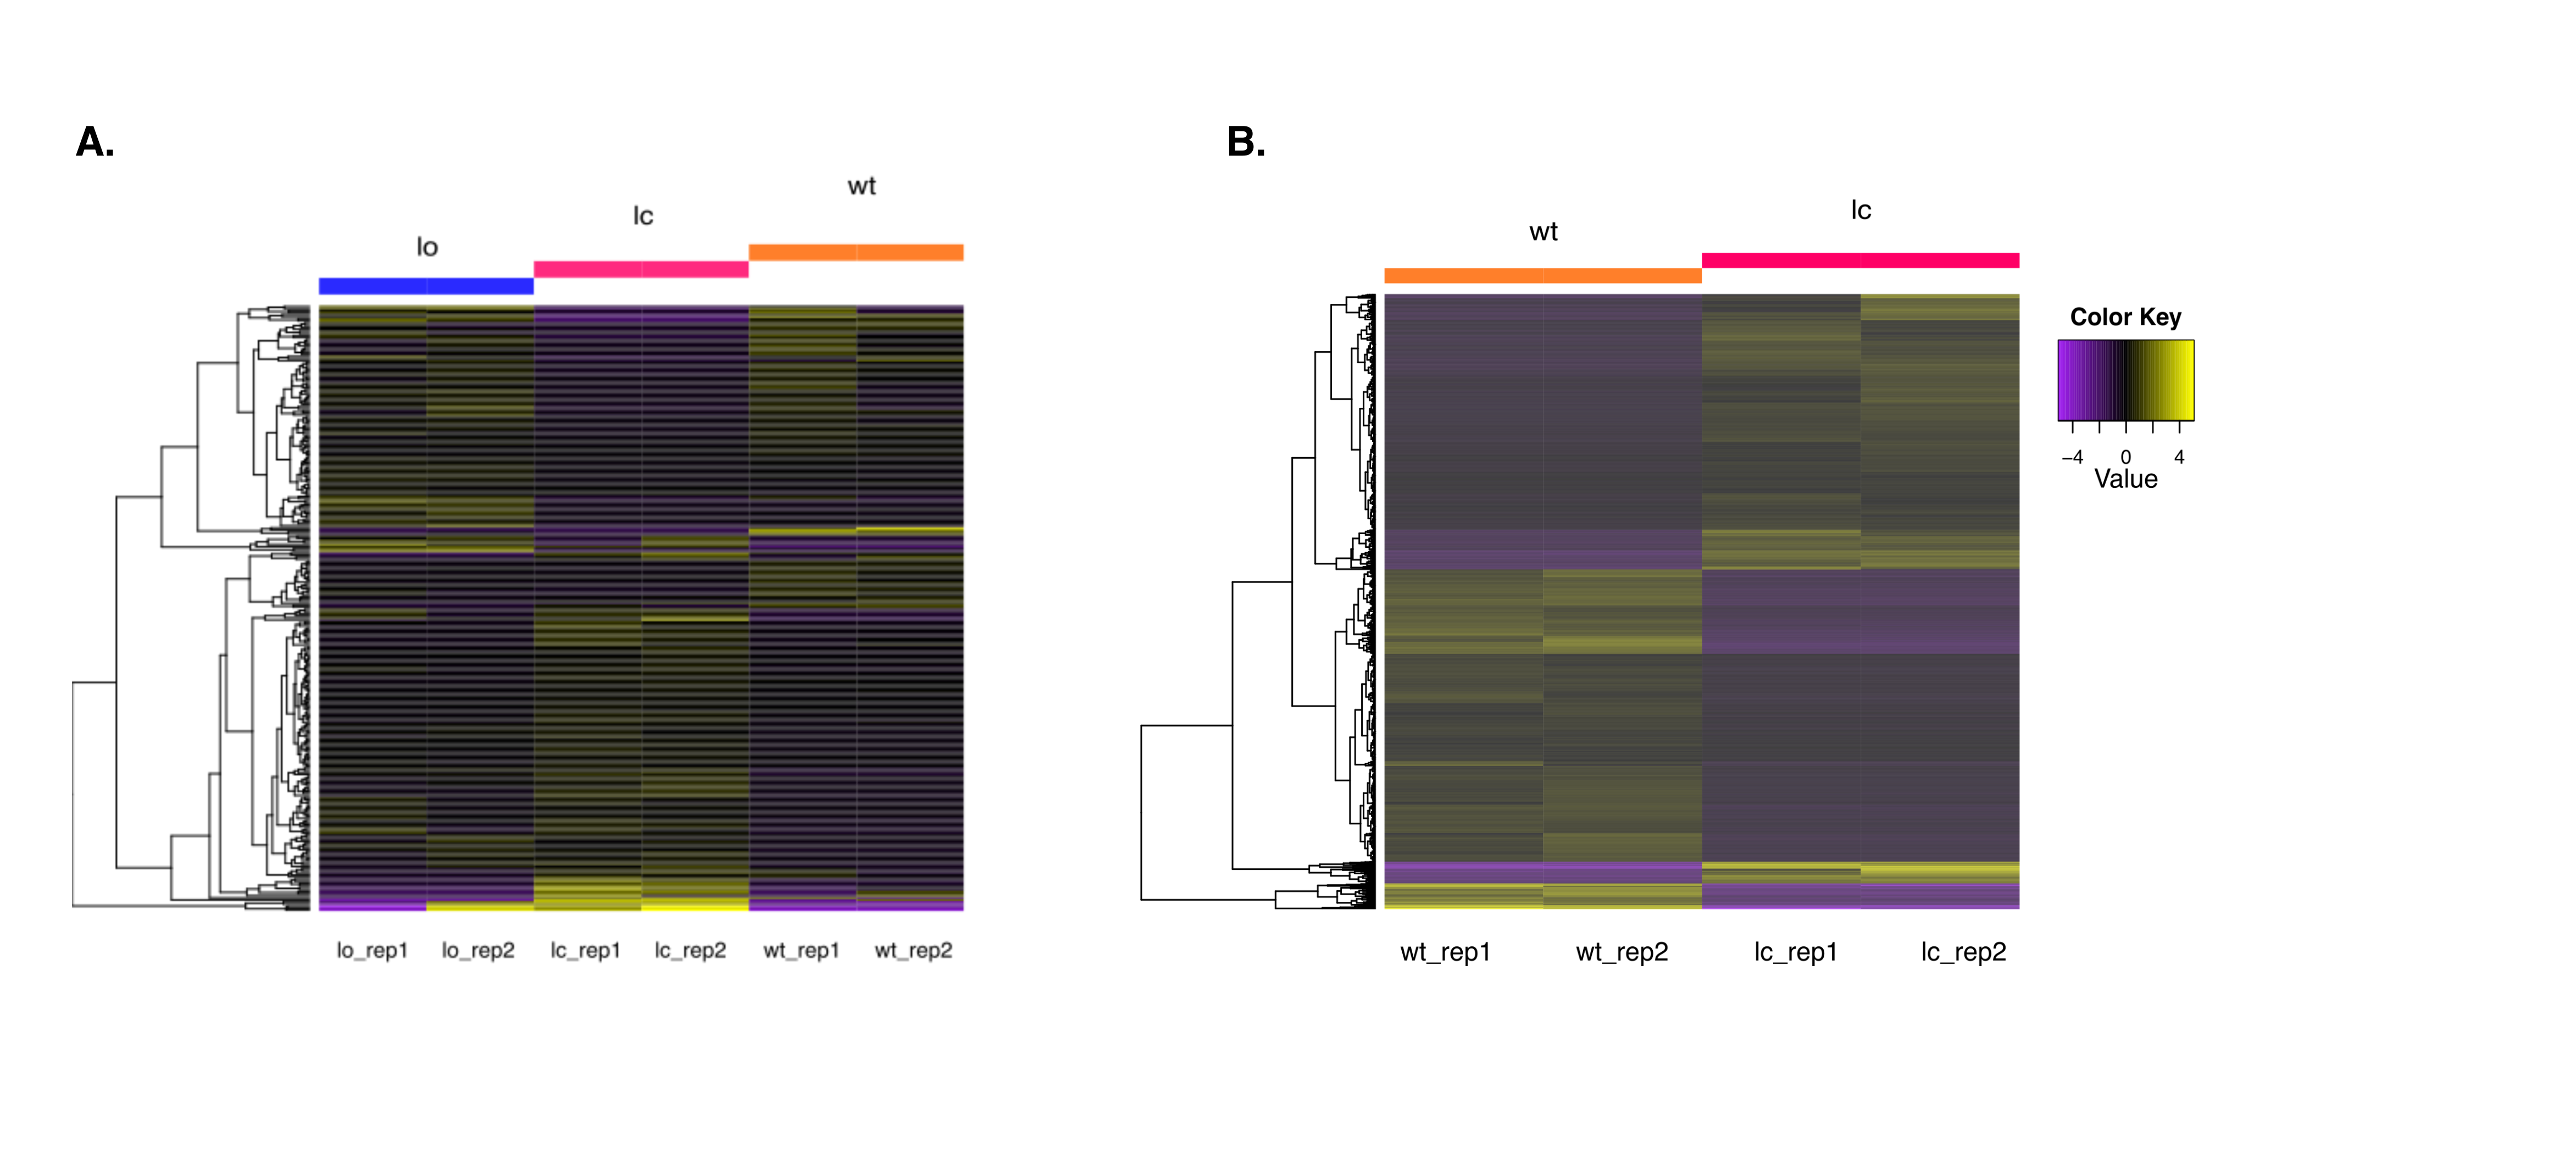
\includegraphics[width=\textwidth]{output/figures/combined-xm-pc-expression-heatmaps-final-project.png}
\caption{Liver transcript-level expression profiles for replicates of (A.) X.mucosus and (B.) P.chirus. Each row is a transcript isoforms and are clustered based on expression similarity in a dendrogram. Columns represent biological replicates of dietary conditions within a species (lo = lab-omnivore; lc = lab-carnivore; wt = wild-type/no dietary intervention). Lowly expressed transcripts (< 0.5 CPM) were not considered.}
\end{figure}

The differential expression analysis revealed distinct responses to diet
in the two species. In P. chirus, a total of 1812 unique transcript
isoforms were differentially expressed between wild-type and
lab-carnivore individuals, indicating a substantial response to dietary
changes. In contrast, X. mucosus exhibited fewer DE transcripts, with a
total of 290 DE transcript isoforms across dietary conditions.
Specifically, 127 transcript isoforms were differentially expressed when
comparing lab-carnivore to lab-omnivore-fed fish, and 182 transcript
isoforms were DE between lab-carnivore and wild-type fish. Only 21
transcript isoforms showed significant differential expression between
lab-omnivore and wild-type X.mucosus (Table 2).

\begin{longtable}[]{@{}
  >{\raggedright\arraybackslash}p{(\columnwidth - 4\tabcolsep) * \real{0.1647}}
  >{\raggedright\arraybackslash}p{(\columnwidth - 4\tabcolsep) * \real{0.3765}}
  >{\raggedright\arraybackslash}p{(\columnwidth - 4\tabcolsep) * \real{0.4588}}@{}}
\toprule\noalign{}
\begin{minipage}[b]{\linewidth}\raggedright
Species
\end{minipage} & \begin{minipage}[b]{\linewidth}\raggedright
Comparison
\end{minipage} & \begin{minipage}[b]{\linewidth}\raggedright
Differentially Expressed Transcripts
\end{minipage} \\
\midrule\noalign{}
\endhead
\bottomrule\noalign{}
\endlastfoot
P.chirus & Lab-Carnivore vs.~Wild-Type & 1812 \\
X.mucosus & Lab-Carnivore vs.~Lab-Omnivore & 127 \\
X.mucosus & Lab-Carnivore vs.~Wild-Type & 182 \\
X.mucosus & Lab-Omnivore vs.~Wild-Type & 21 \\
\end{longtable}

Table 2: EdgeR summarized DE transcripts output for comparisons across
dietary condition within species at thresholds FDR \textless0.01 and FC
\textgreater{} 2.5.

\subsection{Enrichment analysis}\label{enrichment-analysis}

To gain insights into the biological significance of the differentially
expressed isoforms, Gene Ontology (GO) term enrichment analysis was
performed using GOseq. This analysis annotated DE isoforms to
biological, cellular, and molecular terms to uncover functional
categories associated with the transcriptional response to diet in
P.chirus and X.mucosus. GO term analysis of the annotated DE transcripts
in wild-type P.chirus most were enriched in the ``biological processes''
category which included 49 transcripts in adaptive immune response
(\url{GO:0002250}) term, 37 transcripts in immunoglobulin complex
(\url{GO:0019814}) term (Fig 3A). Among the upregulated DE transcripts
enriched in LC P.chirus, 67 were mapped to lipid metabolic processes
(\url{GO:0006629}) term, 36 in transmembrane transporter activity
(\url{GO:0022857}) term, and 29 in response to nutrient levels
(\url{GO:0031667})(Fig 3B).

Generally, fewer transcripts seemed to be differentially expressed
across dietary condition for X. mucosus (Table 2). Between wild-type
X.mucosus relative to LC individuals enriched, broadly, in immune cell
activation and function (\url{GO:0042110}, \url{GO:0046649},
\url{GO:0050776}) (Fig4.A). For DE transcripts unregulated in LC
X.mucosus, 49 mapped to ion binding (\url{GO:0043167}) molecular
function, and 47 transcripts in catalytic activity (\url{GO:0003824})
biological processes (Fig.4B). Additionally, we performed GO enrichment
analysis on a subset of the DE transcripts enriched in LC X.mucosus
relative to LO X.mucosus (Fig.4C). For example, 24 transcripts
upregulated in LC X.mucosus were involved in nitrogen compound metabolic
processes (\url{GO:0006807}), 17 in organic cyclic compound metabolism
(\url{GO:1901360}).

\begin{figure}[htbp]
\centering
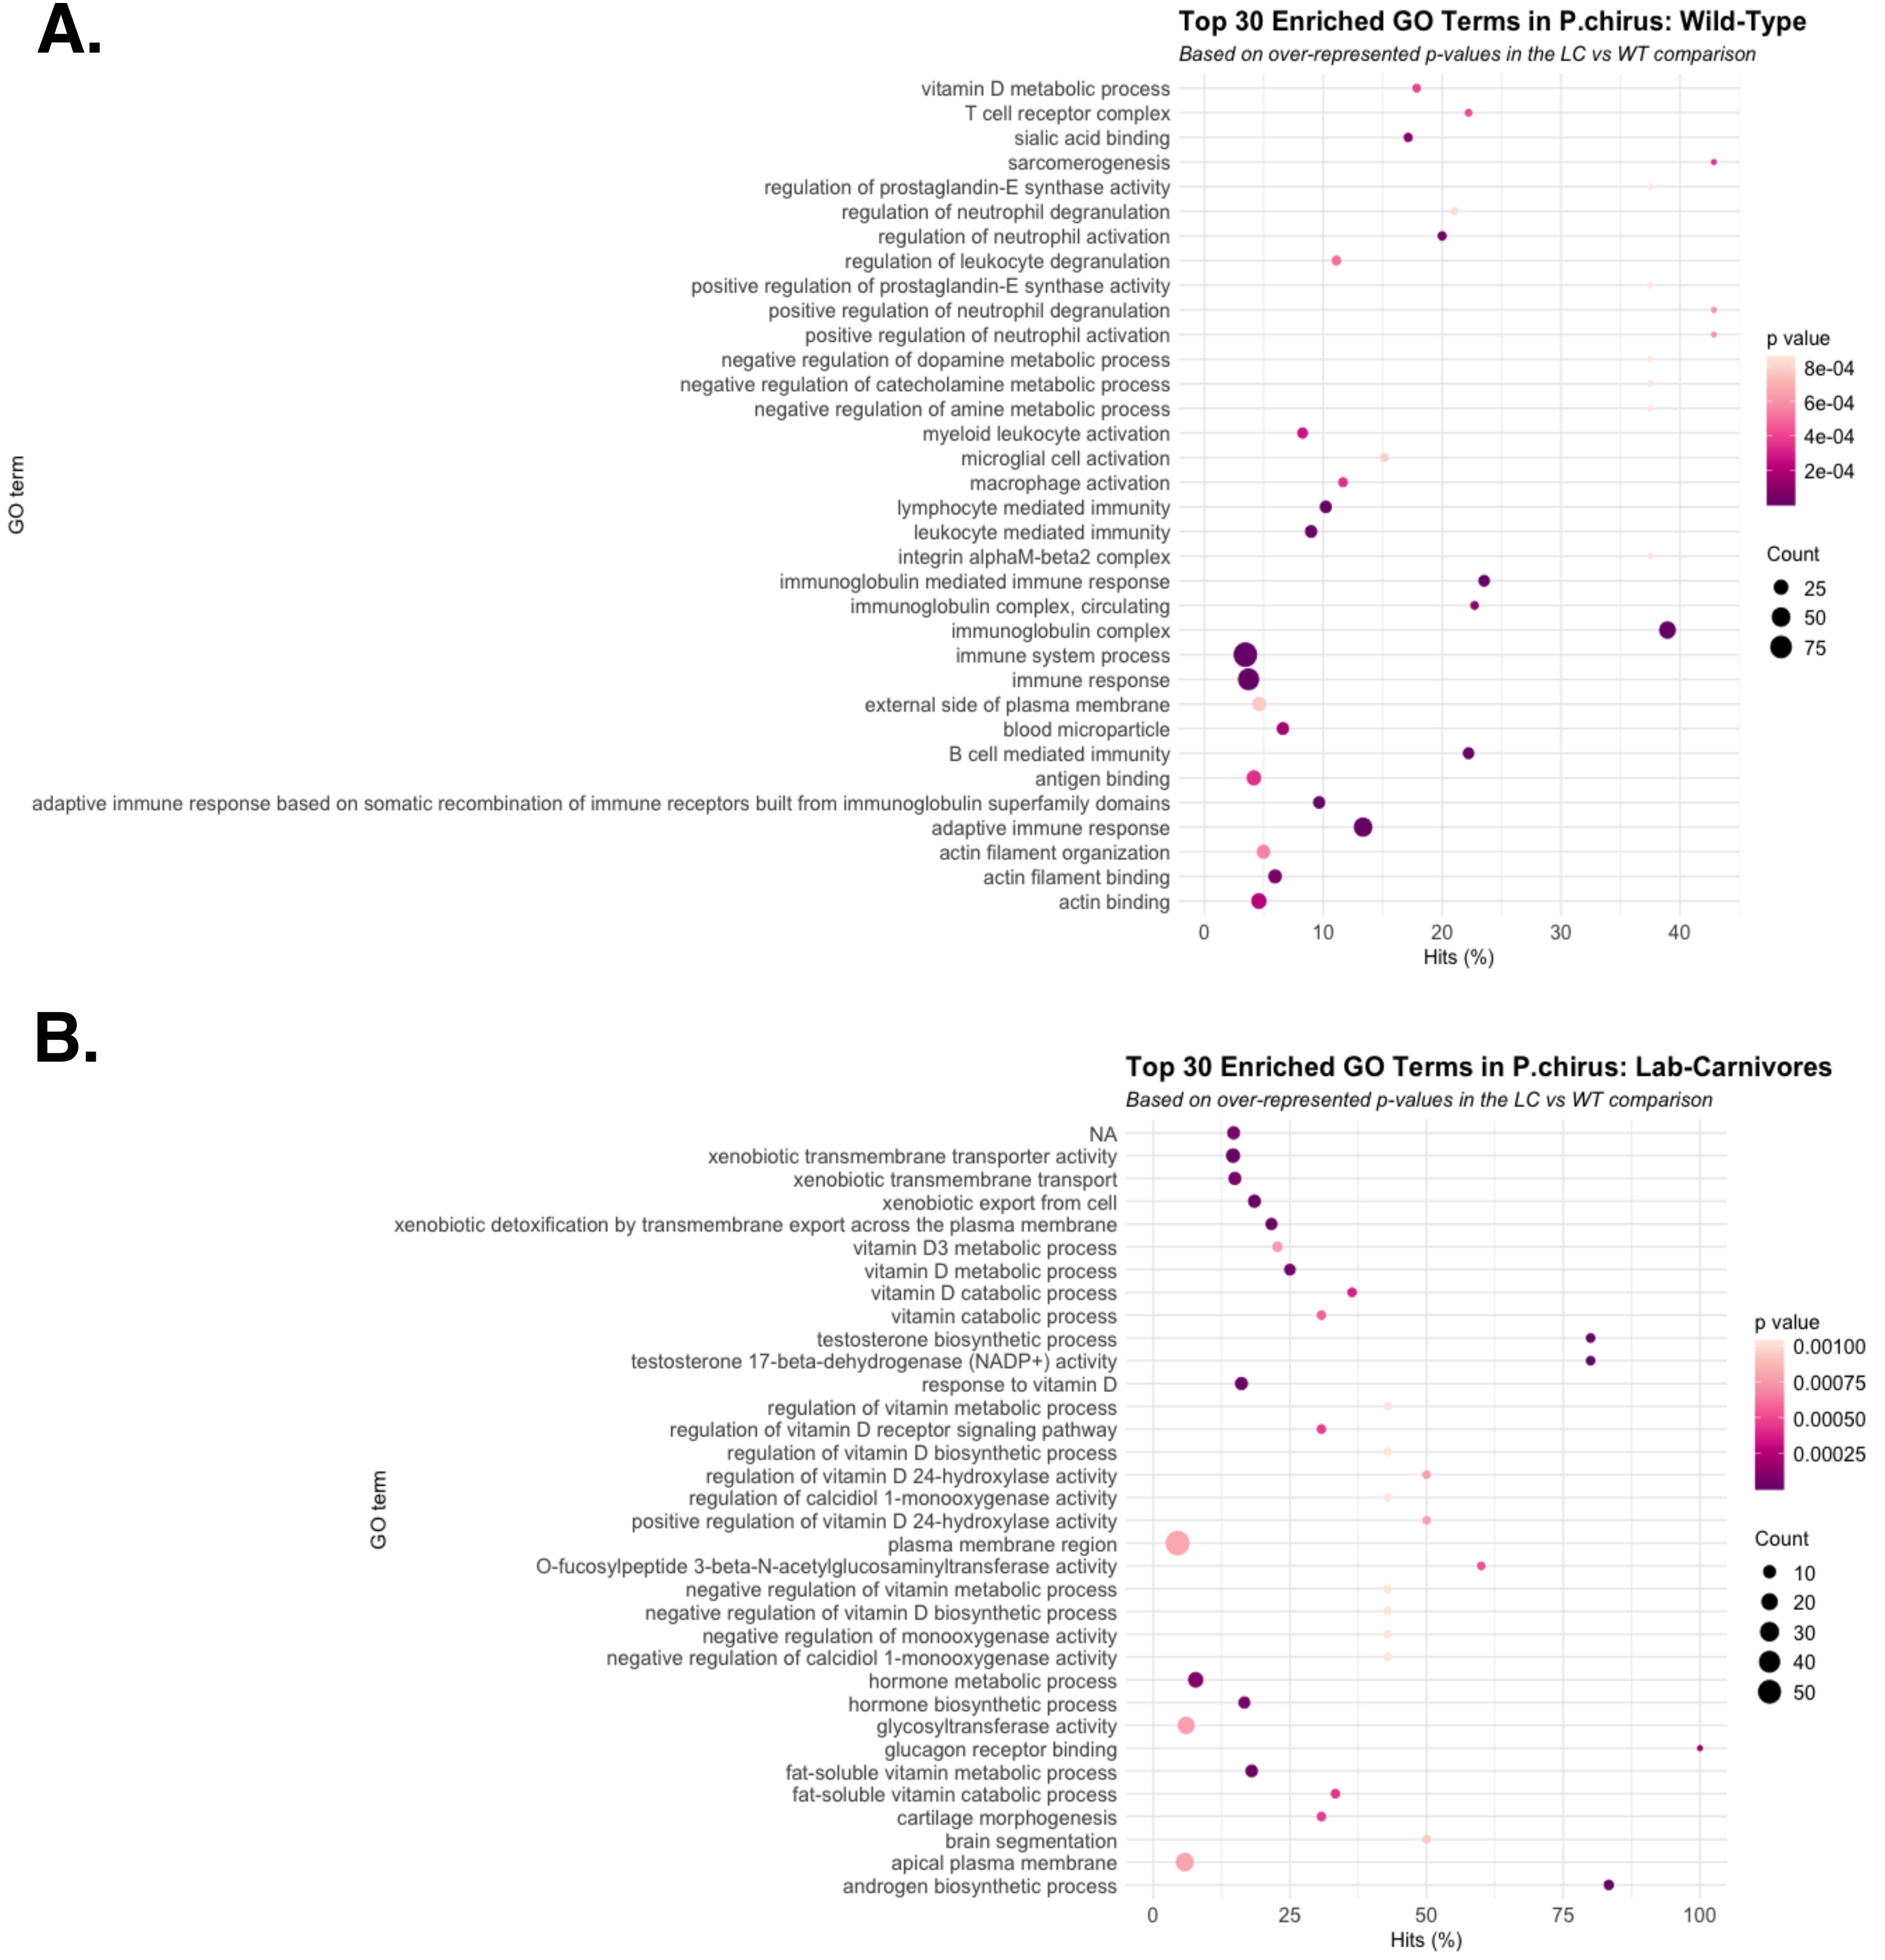
\includegraphics[width=0.85\textwidth]{output/figures/pc_combined_top30_GOseq.png}
\caption{Gene Ontology (GO) term enrichment analysis. An overrepresented p value of < 0.01 was used to pick significantly enriched GO terms in P.chirus.}
\end{figure}

\begin{figure}[htbp]
\centering
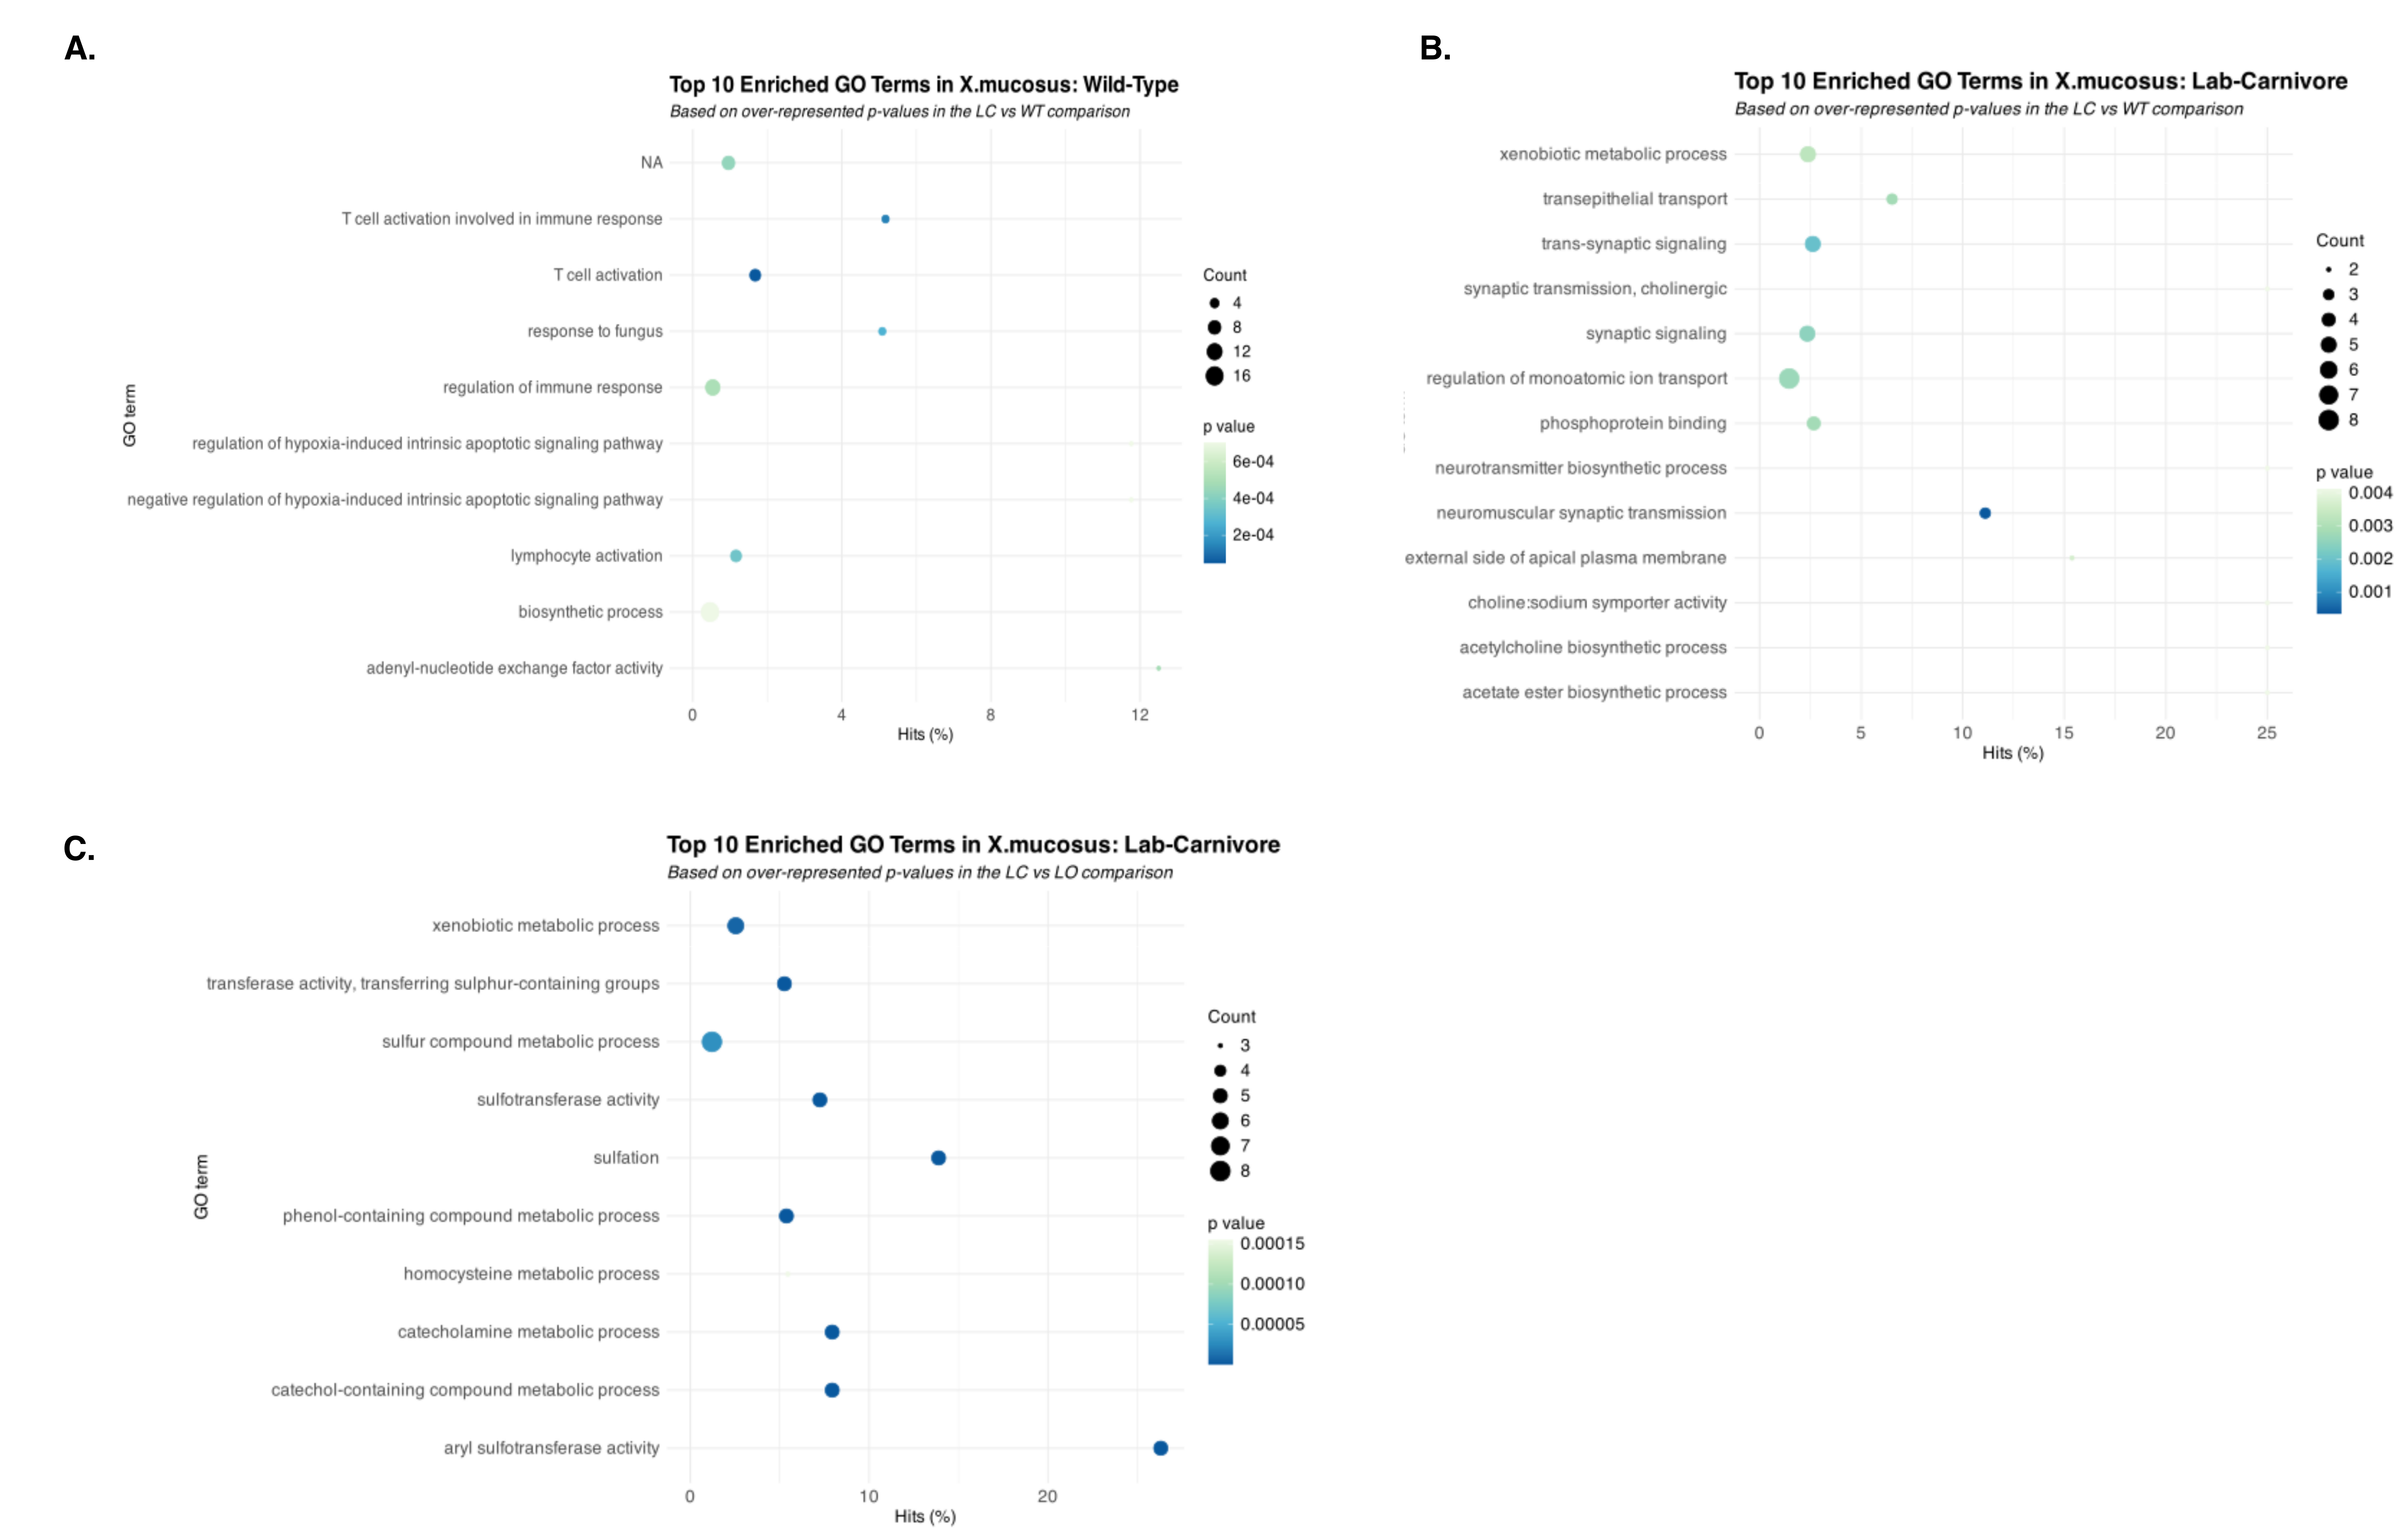
\includegraphics[width=\textwidth]{output/figures/combined-xm-lc_wt_DE_GOseq_enrichment_plot.png}
\caption{Gene Ontology (GO) term enrichment analysis. An overrepresented p value of < 0.01 was used to pick significantly enriched GO terms in X.mucosus.}
\end{figure}

\section{DISCUSSION}\label{discussion}

RNA-Seq analyses have become a reliable method for assessing
transcriptional responses to varying experimental conditions. Previous
gene-level differential expression analysis in P.chirus revealed unique
metabolic flexibility in response to dietary shifts, when compared to
other intertidal Stichaeid species with different diets. Expanding on
this framework, I explored isoform-level changes in both P.chirus and
X.mucosus to determine whether these closely related species exhibited
similar or distinct patterns, driven by their natural dietary
habits.P.chirus, an omnivore, naturally consumes a diet rich in protein
and carbohydrates, while X.mucosus, an herbivore, relies on an
algae-based diet that is low in protein and fat but high in cellulose.

From the original study, when consuming the laboratory carnivore diet
(LC), P.chirus exhibited enriched 13C and 15N signatures in the liver
{[}1{]}. These stable isotopic data indicated that P.chirus was capable
of assimilating more carbohydrates and proteins enriched in the LC diet
compared to wild-type individuals that were not made to stray from their
natural diets. Further comparison of X.mucosus under the wild-type and
LC X.mucosus had upregulated transcripts related to protein metabolic
processes and changes in transmembrane trafficking, suggesting metabolic
switches to processing and transporting nutrients derived from increased
protein intake.

The findings presented here also show that P.chirus exhibits a broader
transcriptional response at the isoform-level in response to a LC diet,
aligning with the earlier gene-level results. In both species, the
wild-type individuals (P.chirus and X.mucosus) exhibited upregulated
transcripts enriched for immune function and cell activation, likely
reflecting the complexity of their natural environments, where exposure
to parasites and microorganisms stimulates adaptive and innate immunity
compared to laboratory conditions.

\subsection{Limitations and future
directions}\label{limitations-and-future-directions}

A limitation of this study was the inability to accurately identify
alternative splicing events in liver transcripts due to the constraints
of short-read sequencing technology. Illumina short reads are limited in
their ability to resolve complex splicing events, and as a result, the
analysis presented here was limited to DE detection and GO enrichment.
However, with the development of new genomic resources for P.chirus, it
will be possible to map differentially expressed transcript isoforms and
assess read coverage and exon structure for protein-coding genes. The
integration of additional bioinformatics tools, such as long-read
sequencing and splicing-aware software, will improve upon one of the
original project goals of understanding alternative splicing and how it
might influence dietary diversification in this species which exhibits
high dietary flexibility under laboratory conditions.

\section{References}\label{references}

Herrera, M.J., Heras, J. \& German, D.P. Comparative transcriptomics
reveal tissue-level specialization towards diet in prickleback fishes.
J. Comp. Physiol. B 192, 275--295 (2022).
\url{https://doi.org/10.1007/s00360-021-01426-1}.

Langmead, B. \& Salzberg, S. Fast gapped-read alignment with Bowtie 2.
Nat. Methods 9, 357--359 (2012).
\url{https://doi.org/10.1038/nmeth.1923}.

Chen, S., Zhou, Y., Chen, Y. \& Gu, J. fastp: an ultra-fast all-in-one
FASTQ preprocessor. Bioinformatics 34, i884--i890 (2018).
\url{https://doi.org/10.1093/bioinformatics/bty560}.

Li, B. \& Dewey, C.N. RSEM: accurate transcript quantification from
RNA-Seq data with or without a reference genome. BMC Bioinformatics 12,
323 (2011). \url{https://doi.org/10.1186/1471-2105-12-323}.

Grabherr, M.G. et al.~Full-length transcriptome assembly from RNA-Seq
data without a reference genome. Nat. Biotechnol. 29, 644--652 (2011).
\url{https://doi.org/10.1038/nbt.1883}.

Robinson, M.D., McCarthy, D.J. \& Smyth, G.K. edgeR: a Bioconductor
package for differential expression analysis of digital gene expression
data. Bioinformatics 26, 139--140 (2010).
\url{https://doi.org/10.1093/bioinformatics/btp616}.

Andrews, S. FastQC: a quality control tool for high throughput sequence
data. Available at:
\url{http://www.bioinformatics.babraham.ac.uk/projects/fastqc} (2010).

Ewels, P., Magnusson, M., Lundin, S. \& Käller, M. MultiQC: summarize
analysis results for multiple tools and samples in a single report.
Bioinformatics 32, 3047--3048 (2016).
\url{https://doi.org/10.1093/bioinformatics/btw354}.

Brian, H. \& Papanicolaou, A. Transdecoder (Find Coding Regions Within
Transcripts). Retrieved from \url{http://transdecoder.github.io} (n.d.).

Bryant, D.M. et al.~A tissue-mapped axolotl de novo transcriptome
enables identification of limb regeneration factors. Cell Rep.~18,
762--776 (2017). \url{https://doi.org/10.1016/j.celrep.2017.01.002}.

Young, M.D., Wakefield, M.J., Smyth, G.K. et al.~Gene ontology analysis
for RNA-seq: accounting for selection bias. Genome Biol. 11, R14 (2010).
\url{https://doi.org/10.1186/gb-2010-11-2-r14}.

\section{Supplemental material}\label{supplemental-material}

\begin{figure}[htbp]
\centering
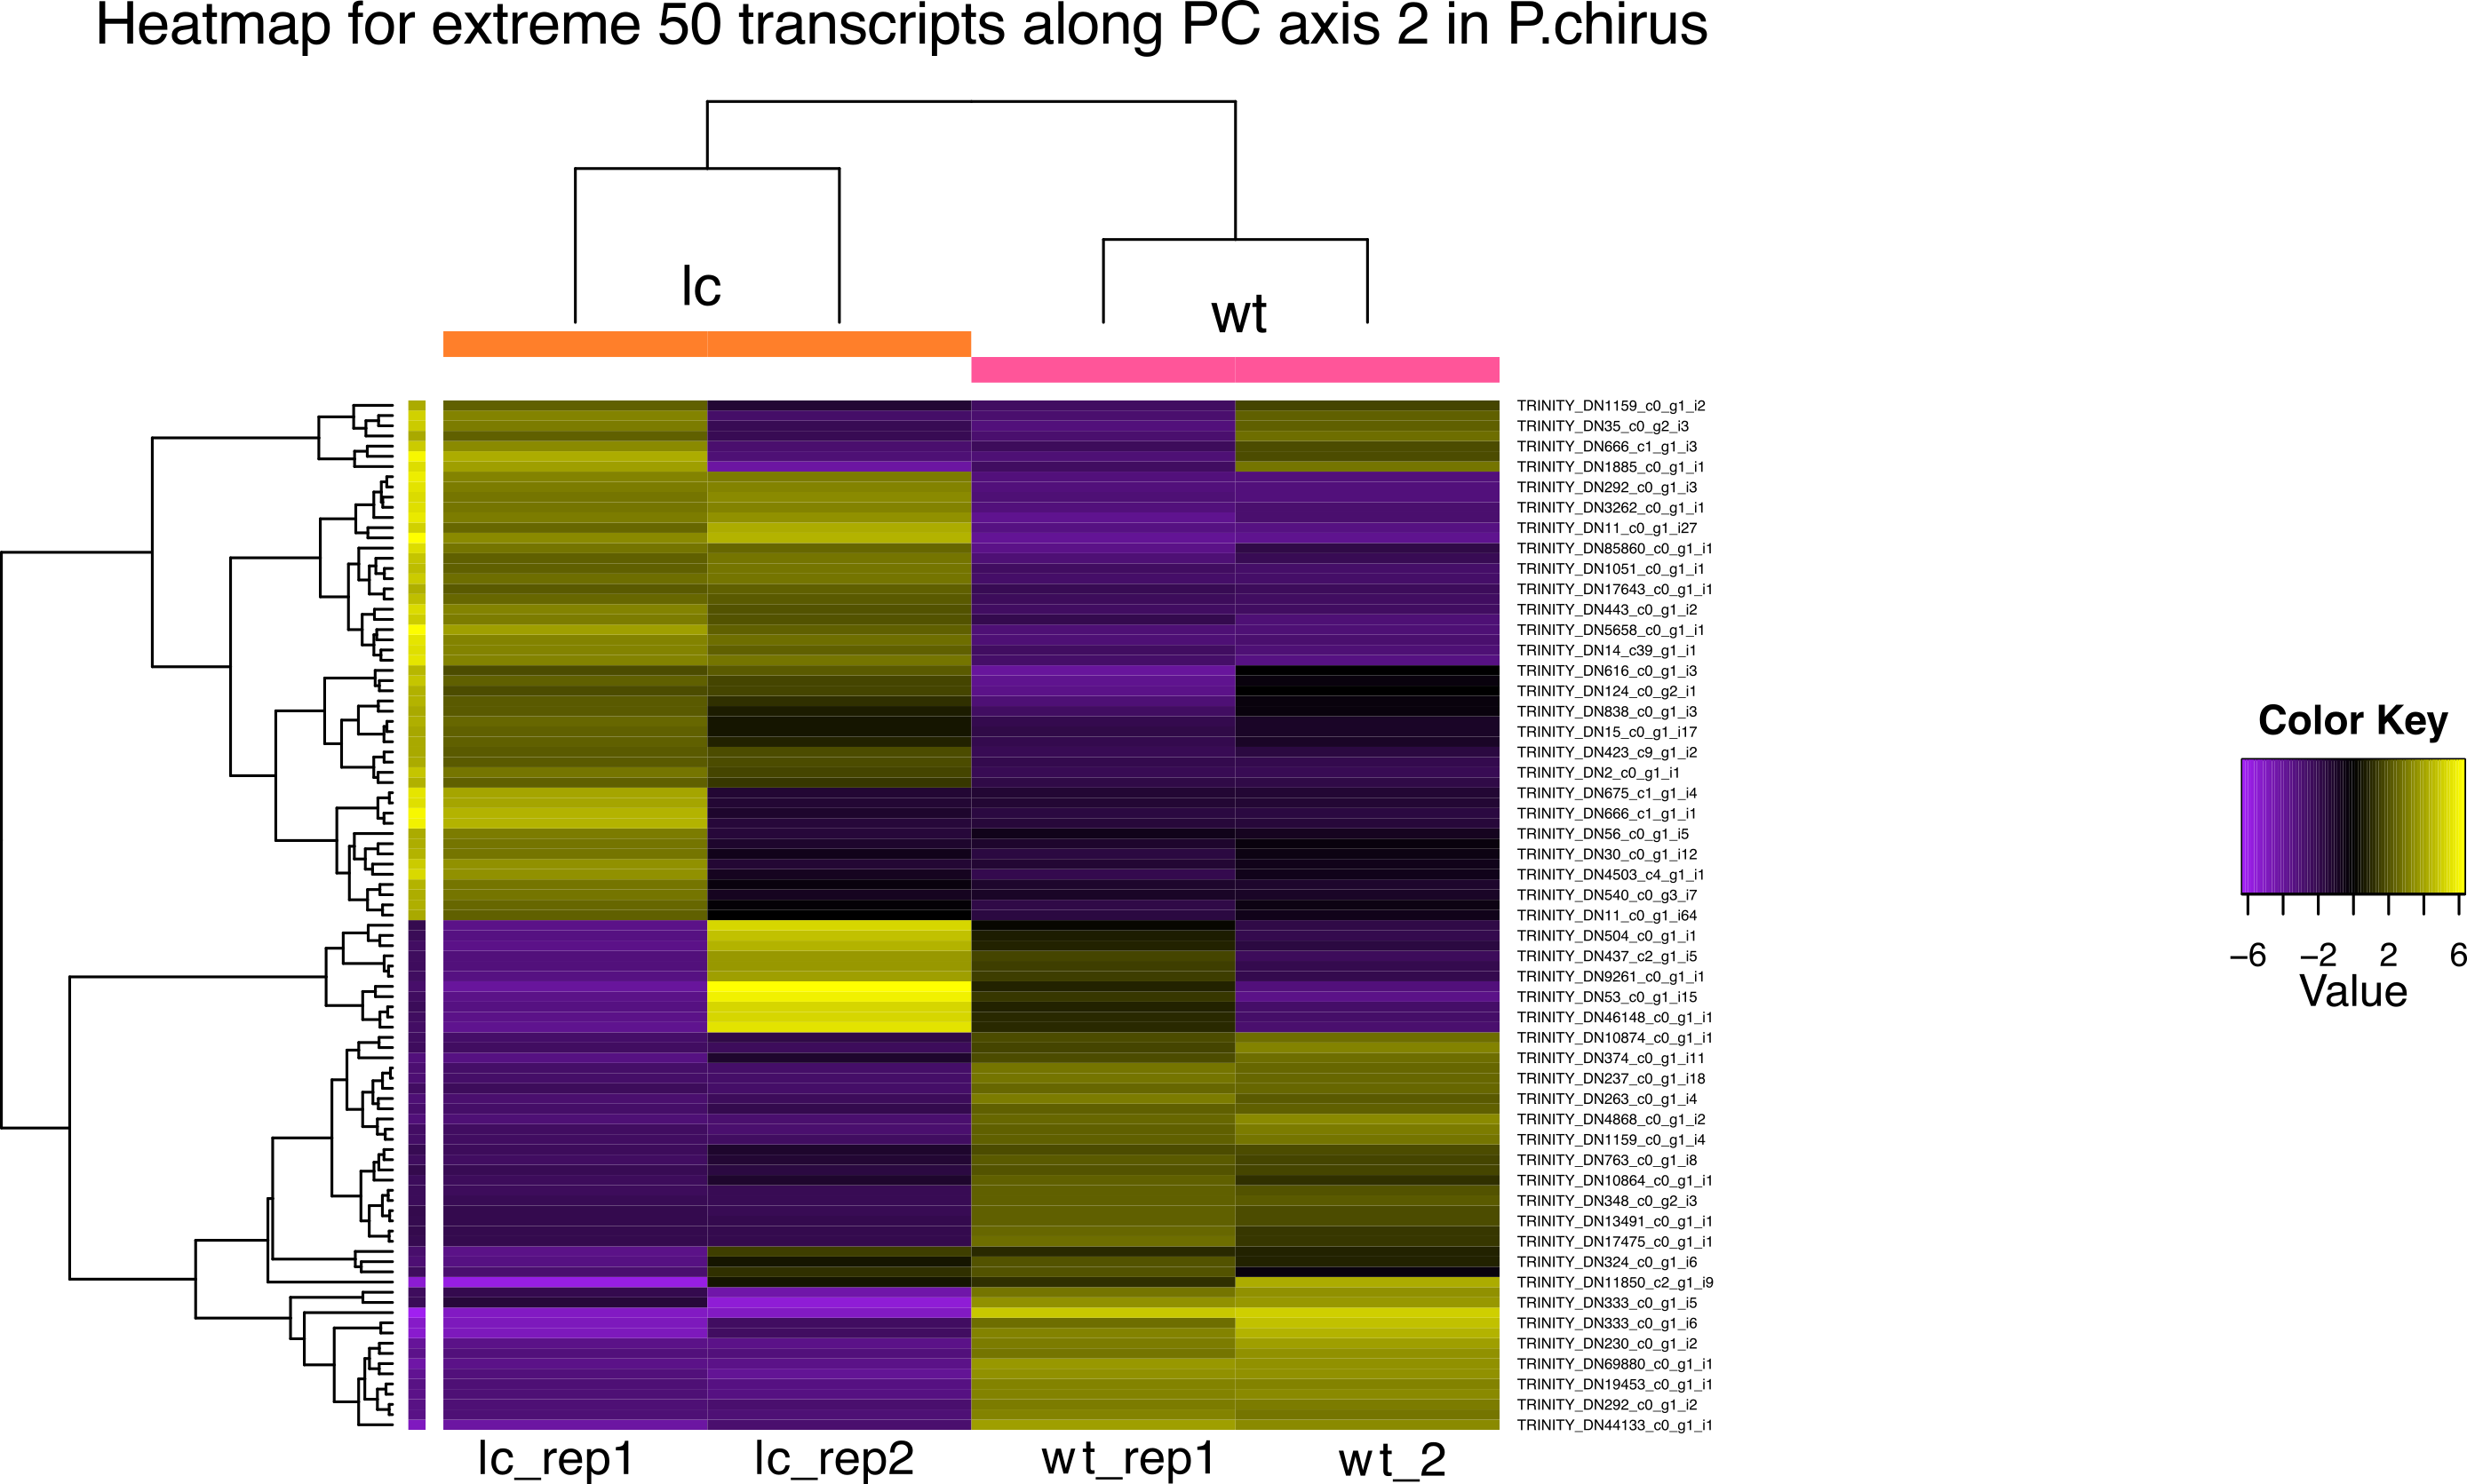
\includegraphics[width=0.85\textwidth]{output/figures/pc_and_xm_TMM_EXPR.minRow10.log2.centered.prcomp.extreme50.PC2.components.png}
\caption{Subset heatmap for 50 extreme transcripts driving variation along the second axis of variation PC 2 for P.chiurs.}
\end{figure}





\newpage
\singlespacing 
\bibliography{ee282\_library.bib}

\end{document}
